\section{Analyse der Energiespektren}
Da leider nicht alle Messungen über die selbe Zeit aufgenommen wurden, mussten diese über die Messdauer normiert werden, es wurden also immer die Zählraten anstatt der Counts verwendet. Diese Normierung wurde immer nach 
Berechnung der  statistischen Fehler des Datensatzes über die Formel \ref{zählfehler} durchgeführt. Die Fehler wurden nach der Formel \ref{fehlerfortp} fortgepflanzt.
\begin{equation}
\Delta_N = \sqrt{N}
\label{zählfehler}
\end{equation}
\begin{equation}
	\Delta_\frac{N}{t} = \frac{\Delta_N}{t} 
	\label{fehlerfortp}
\end{equation}
\subsection{Untergrund}
Zu Beginn wurde die Untergrundmessung ausgewertet, da diese benötigt wird um alle weiteren Messungen zu korrigieren. Es wurde statt einer langen Messung zwei kürzere aufgenommen, was durch addieren der Counts pro Bin behoben wurde.
Für die resultierende Datenreihe wurden wie oben beschrieben die statistischen Fehler berechnet und die Normierung durchgeführt. Die zur Hintergrundkompensation genutzte Datenreihe ist in Abbildung \ref{untergrund} zu sehen.
\begin{figure}[h]
	\centering
	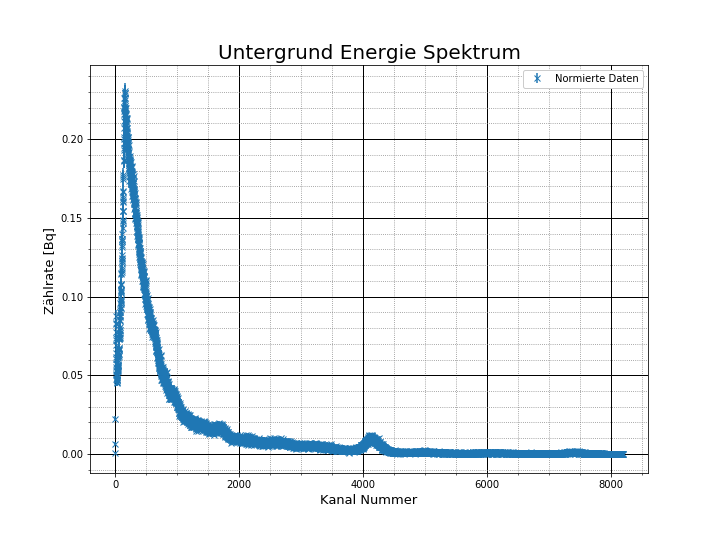
\includegraphics[scale=0.5]{Bilder/untergrund}
	\caption[Normalisierter Hintergrund]{\small Im Bild ist der Hintergrund Datensatz zu sehen. Es wurde die Zählrate pro Kanal aufgetragen. }
	\label{untergrund}
\end{figure}
\subsection{Energiekalibrierung}
Um den aktuellen Zusammenhang zwischen Kanälen des MCA und Energie der Detektierten $\gamma$ Photonen zu bestimmen, wurden die bekannten Peaks der Spektren von Natrium, Cobalt und Europium verwendet. Die so gewonnenen Zusammenhänge wurden auf den gesamten Bereich extrapoliert. Es wurden immer die statistischen Fehler in den Fits berücksichtigt.
\subsubsection{Natrium}
Für das Spektrum der $^{22}Na$ Probe wurden zwei Peaks erwartet, die Intensität des mit niedrigerer Energie einen deutlich größer als die des höher energetischen Peaks. Genau dies wurde beobachtet, somit konnten erfolgreich die Kanal-Energie Zusammenhänge für den 511 und 1275 keV Peak bestimmt werden. Hierzu wurden zunächst Analog zur Hintergrundmessung die statistischen Fehler bestimmt und die Counts in die Zählrate umgerechnet. 
Anschließend wurde eine Gaußkurve (nach Gleichung \ref{gaussian}) mittels Python \cite{SciPy_Opti} gefittet. Die Mittelpunkte der Peaks ($\mu$), welche für die Kalibrierung verwendet wurden sind der Abbildung \ref{natrium} zu entnehmen. 
\begin{figure}[h]
	\centering
	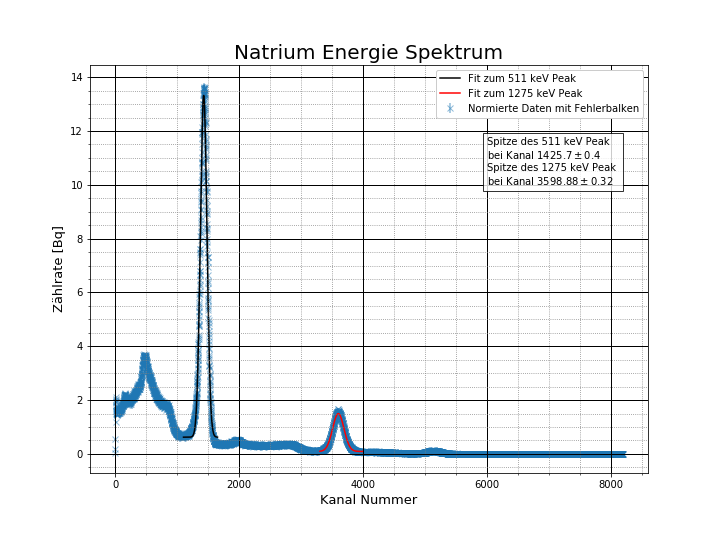
\includegraphics[scale=0.5]{Bilder/Natrium}
	\caption[Natriumspektrum mit Peaks]{\small Im Bild ist das Natrium Spektrum zu sehen. Es wurde die Zählrate pro Kanal aufgetragen und die Fits eingezeichnet. Zusätzlich sind die $\mu$ Werte der gefitteten Kurven eingetragen.}
	\label{natrium}
\end{figure}
\begin{equation}
f(x,\mu, \sigma, A, B) = B + A \cdot e ^{-\frac{(x - \mu) ^ 2}{2 \cdot \sigma ^ 2}}
\label{gaussian}
\end{equation}
\subsubsection{Cobalt}
Für das zur Kalibrierung verwendete Spektrum von $^{60}Co$ wurde analog zur Analyse des Natriumspektrums vorgegangen. Hier wurden zwei Peaks mit den Energien 1173 und 1333 keV erwartet. Diese konnten ohne größere Probleme gefunden und gefittet werden. Die relevanten Werte sind aus Abbildung \ref{cobalt} zu entnehmen. 
\begin{figure}[h]
	\centering
	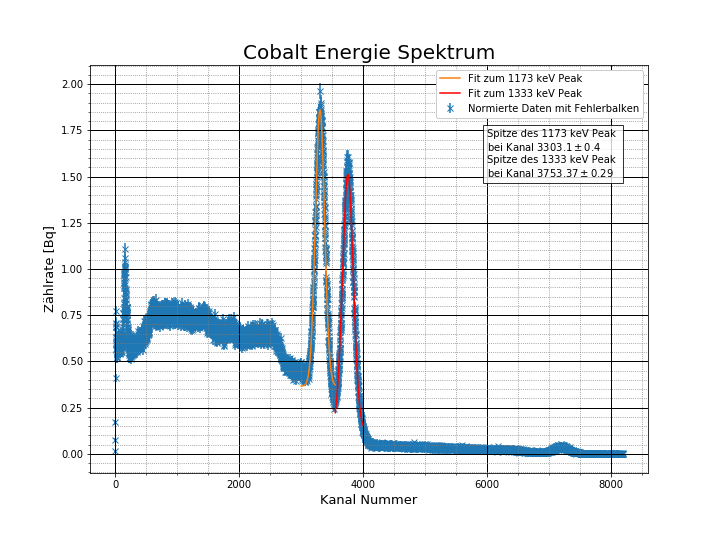
\includegraphics[scale=0.5]{Bilder/Cobalt}
	\caption[Cobalt Spektrum mit Peaks]{\small Im Bild ist das Cobalt Spektrum zu sehen. Es wurde die Zählrate pro Kanal aufgetragen und die Fits eingezeichnet. Zusätzlich sind die $\mu$ Werte der gefitteten Kurven eingetragen.}
	\label{cobalt}
\end{figure}
\subsubsection{Europium}
Durch die höhere Komplexität des Zerfalls von $^{152}Eu$ wurden im gemessenen Spektrum viele Peaks aufgezeichnet. Mit der Natriummessung als Referenz konnten die ungefähren Kanäle für die Energien von 122 und 344 keV bestimmt werden und analog zu den anderen beiden Messungen die Auswertung durchgeführt werden. Die relevanten Werte sind aus Abbildung \ref{europium} zu entnehmen. Durch

\begin{figure}[h]
	\centering
	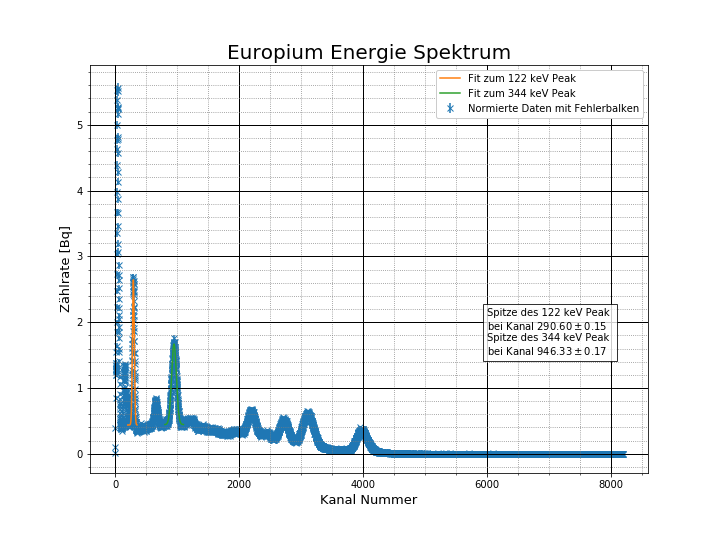
\includegraphics[scale=0.5]{Bilder/Europium}
	\caption[Europium Spektrum mit Peaks]{\small Im Bild ist das Europium Spektrum zu sehen. Es wurde die Zählrate pro Kanal aufgetragen und die Fits eingezeichnet. Zusätzlich sind die $\mu$ Werte der gefitteten Kurven eingetragen.}
	\label{europium}
\end{figure}
\subsubsection{Energieeichung}
Die in den vorherigen Abschnitten gewonnenen Energie-Kanal paare wurden nun aufgetragen und eine Linie wurde gefittet. Diesen Fit und die Parameter können in Abbildung \ref{energiekali} gefunden werden. Beim fit wurden die Fehler der Kanalnummer berücksichtigt, da die Energien ohne Fehler angenommen werden.

\begin{figure}[h]
	\centering
	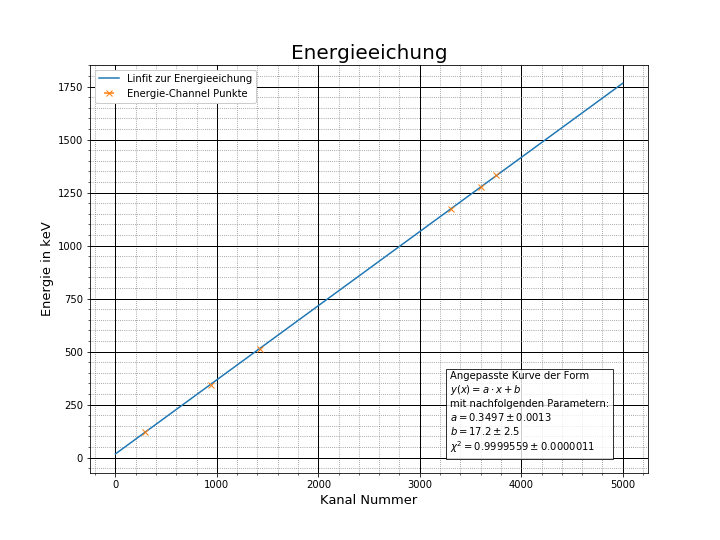
\includegraphics[scale=0.5]{Bilder/Energieeichung}
	\caption[Energieeichung]{\small Hier wurden die Kanal-Energie Paare aufgetragen und eine Kurve gefittet. Die Funktion und deren Parameter sowie die Güte sind zusätzlich eingetragen. }
	\label{energiekali}
\end{figure}

\subsection{Thorium Spektrum}
Das $^{228}Th$ Spektrum ist viel komplexer als die vorherigen. Es wurden 9 Peaks gefittet, wobei die Abbildungen hierzu im Anhang zu finden sind. Der 3. Peak ist ein Doppelpeak, sodass nicht die übliche Funktion (\ref{gaussian}) sondern eine Kombination aus zwei solcher Funktionen (\ref{doppelgaus}) gefittet wurde. Es wurde auch weiterhin Python \cite{SciPy_Opti} verwendet. Es wurden weiterhin die Statistischen Fehler berücksichtigt, da die Fehler auf die Energie viel kleiner sind.
\begin{equation}
	f(x,\mu,\mu_2,\sigma,\sigma_2,A,A_2,B) = 
	 A \cdot e ^{-\frac{(x - \mu) ^ 2}{2 \cdot \sigma ^ 2}} + 
	 A_2 \cdot e ^{-\frac{(x - \mu_2) ^ 2}{2 \cdot \sigma_2 ^ 2}} + 
	 B
	 \label{doppelgaus}
\end{equation}
In Abbildung \ref{thorium} ist das gesamte Thorium Spektrum in Logarithmischer Skala aufgetragen. Anschließend wurden kleinere Ausschnitte aufgetragen, dass die einzelnen Peaks besser erkennbar sind. Im Spektrum bis 500 keV (Abb. \ref{th_500}) wurden alle 5 Peaks gefittet. Im Spektrum von 500 bis 1000 keV (Abb. \ref{th_1000}) wurden alle 3 gut sichtbaren Peaks gefittet. Am Ende wurde noch der gut sichtbare Peak bei $\approx 3700$ keV gefittet. Die Energien der gefitteten Peaks sind auf den Abbildungen der jeweiligen Peaks in der Zuordnung zu finden
Die Mittelpunkte ($\mu$) der gefitteten Kurven wurden in der Tabelle \ref{ergebnisse_thorium} eingetragen. 
\begin{figure}[h]
	\centering
	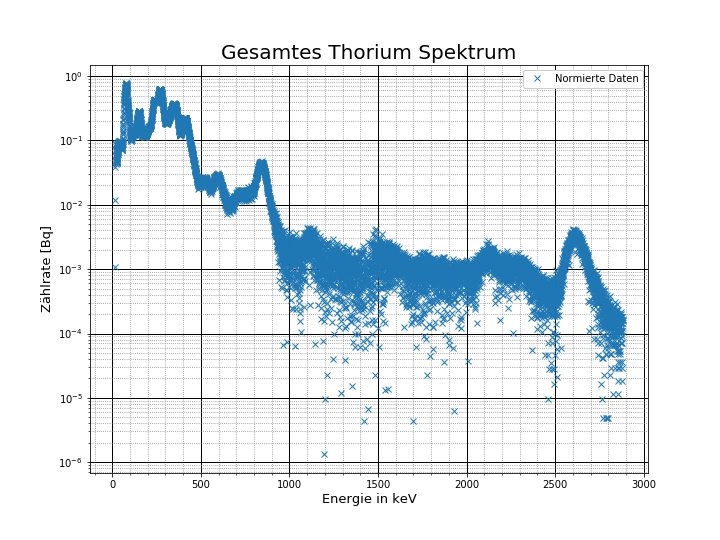
\includegraphics[scale=0.7]{Bilder/Th_ganz}
	\caption[Gesamtes Thorium Spektrum]{\small Thorium Spektrum in log. Skala, sodass alle Peaks mit stark variierenden Zählraten sichtbar sind.}
	\label{thorium}
\end{figure}

\begin{figure}[h]
	\centering
	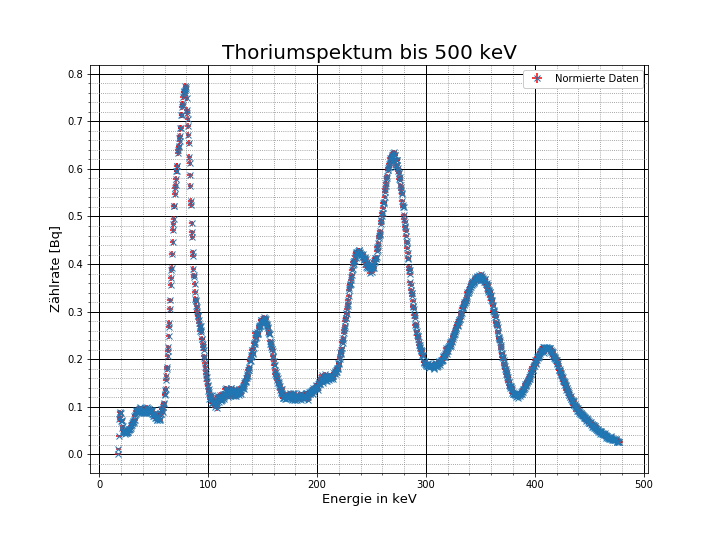
\includegraphics[scale=0.7]{Bilder/Th_1}
	\caption[Thorium Spektrum bis 500 keV]{\small Thorium Spektrum in lin. Skala bis 500 keV. Es sind die Peaks 1 bis 5 sichtbar, wobei Peak 3 ein Doppelpeak ist. Es wurde die Fehlerbalken zur Übersicht nicht bei allen Punkten eingezeichnet, die Energiefehler sind außerdem zu klein um dargestellt zu werden.}
	\label{th_500}
\end{figure}

\begin{figure}[h]
	\centering
	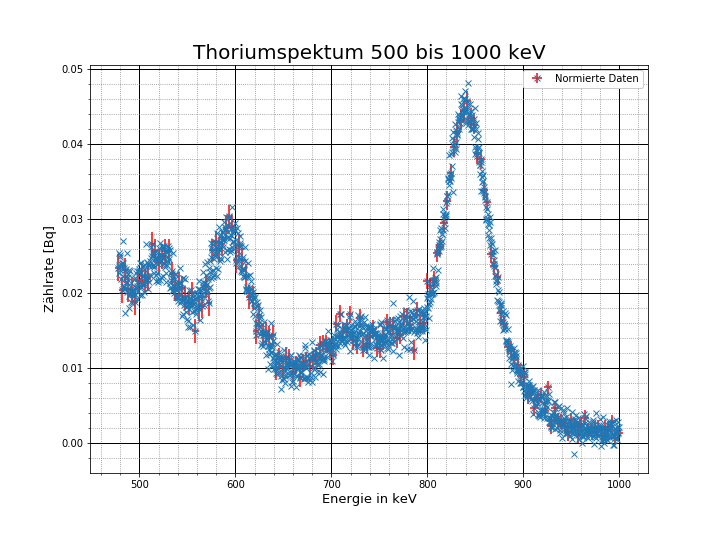
\includegraphics[scale=0.7]{Bilder/Th_2}
	\caption[Thorium Spektrum 500 bis 1000 keV]{\small Thorium Spektrum in lin. Skala von 500 bis 1000 keV. Es sind die Peaks 6 bis 8 sichtbar.
	Es wurde die Fehlerbalken zur Übersicht nicht bei allen Punkten eingezeichnet, die Energiefehler sind außerdem zu klein um dargestellt zu werden.}
	\label{th_1000}
\end{figure}
 \FloatBarrier
\subsection{Identifizierung der gemessenen Peaks}
Im Anschluss an die Bestimmung der Energien von den 10 verschiedenen Peaks (vgl. oben) wurden diese mit der Zerfallsreihe von Thorium verglichen um so die Übergänge zu Identifizieren bei welchen die gezählten $\gamma$ Photonen erzeugt wurden.
\subsubsection{Peak 1}
Peak 1 wurde bei einer Energie von $77.26\pm0.10\,$keV gefittet. 
Beim Blick auf Abbildung \ref{p1} ist auffällig, dass der Peak unsauber ist, als ob er bei ca. 72 keV einen weiteren Peak besitzt, was den gesamten Fit verzieht. Das echte Maximum von Peak 1 liegt außerdem bei einer deutlich höheren Energie als das Maximum des Fits. Deshalb wird es als sinnvoll empfunden, einen anderen Mittelpunkt und ein größerer Fehler auf diesen Wert angenommen: Der neue Wert liegt nun bei $80\pm5\,$keV.\par
Wahrscheinlich handelt es sich hier um den Übergang von Thorium zu Radium mit Energie 84.373 keV \cite{Thorium}. Von der Energie würde zusätzlich noch der Übergang Thorium zu Radium bei 74.4 keV, möglich sein, was vermutlich den Peak leicht zu einer niedrigeren Energie verschob.
\begin{figure}[h]
	\centering
	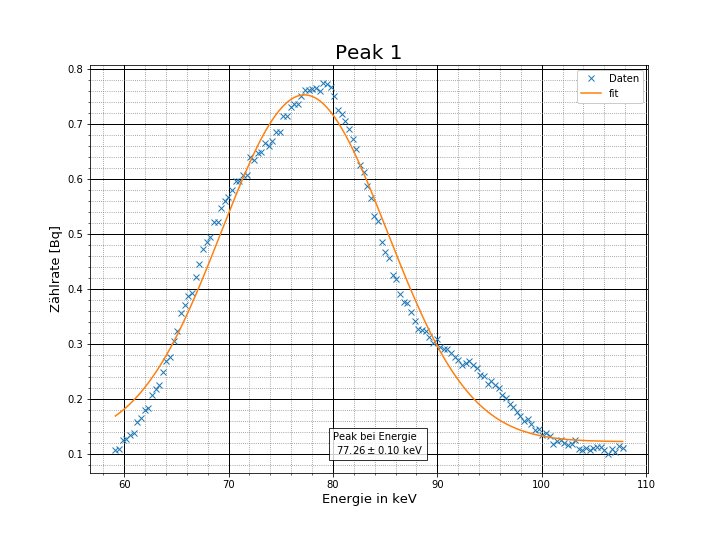
\includegraphics[scale=0.7]{Bilder/Anhang/P1}
	\caption[Thorium Peak 1]{\small Die verwendeten Daten von Peak 1, dessen Fit und der Mittelpunkt des Fits.}
	\label{p1}
\end{figure}
\subsubsection{Peak 2}
Das Maximum von Peak 2 wurde bei einer Energie von $149.67\pm0.08\,$keV gefittet. Dies ist aus Abbildung \ref{p2}. Durch die hohe Streuung in der Umgebung des Maximums wird es für sinnvoll gehalten, den Fehler zu vergrößern: Somit gilt nun für den Mittelpunkt des Fits die Energie von $150\pm5\,$keV.\par
Bei dieser Energie liegt kein direkter Peak vor, aber es existieren die Übergänge 131.612 keV  und 166.41 keV  von Thorium zu Radium \cite{Thorium} . Deshalb wird vermutet, dass der gemessene Peak eine Kombination von beiden sei, welche wegen den Unterschiedlichen Wahrscheinlichkeiten der Übergänge nicht mittig zwischen ihnen liegt, sondern etwas näher an 166.41 keV.
\begin{figure}[h]
	\centering
	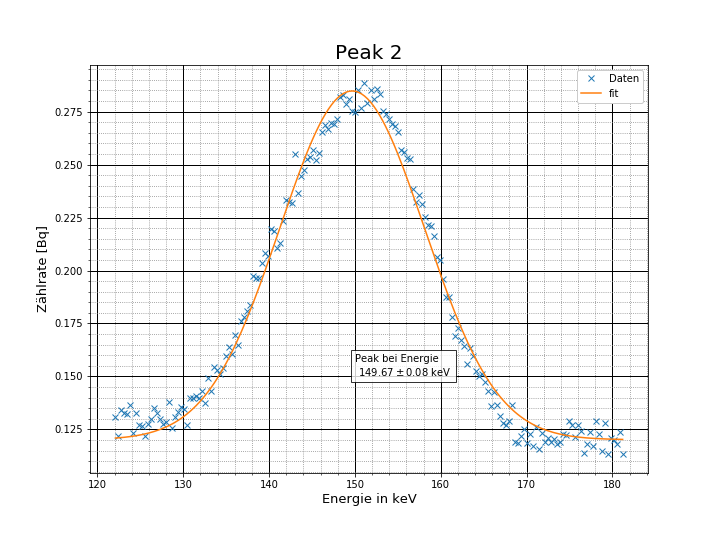
\includegraphics[scale=0.7]{Bilder/Anhang/P2}
	\caption[Thorium Peak 2]{\small Die verwendeten Daten von Peak 2, dessen Fit und der Mittelpunkt des Fits.}
	\label{p2}
\end{figure}

\subsubsection{Peak 3}
Peak 3 war ein Kombinationspeak. Deshalb werden die beiden Komponenten von ihm einzeln als 3.1 und 3.2 betrachtet. Dies ist alles in Abbildung \ref{p3} zu sehen.\\
Das gefittete Maximum von Peak 3.1 liegt bei $237.62\pm0.10\,$keV. Da der Kombinationsfit in dieser Region deutlich über der Mehrheit der Punkte liegt, wurde es für sinnvoll erachtet den Fehler auf einen größeren Wert festzulegen: Für Peak 3.1 gilt nun $238\pm2\,$keV.\\
Das gefittete Maximum von Peak 3.2 liegt bei $269.88\pm0.06\,$keV. Da hier am Peak eine gewisse Streuung der Messpunkte vorliegt, wird auch ein vergrößerter Fehler angenommen: Somit gilt für Peak 3.2 nun eine Energie von
$270\pm1\,$keV. Vermutlich spielen hier außerdem Überlagerungen von Comptoneffekten der darüberlegenden Peaks eine Rolle, weshalb zusätzlich systematische Fehler anzunehmen sind. \cite{staatsex_szinti} \par
Für die Energie zu Peak 3.1 passt der Übergang von Blei zu Bismut \cite{Blei} mit einer Energie von 238.632 keV. Für Peak 3.2 passt der Übergang von Thallium zu Blei bei 277.37 keV \cite{Thallium} am Wahrscheinlichsten. 


\begin{figure}[h]
	\centering
	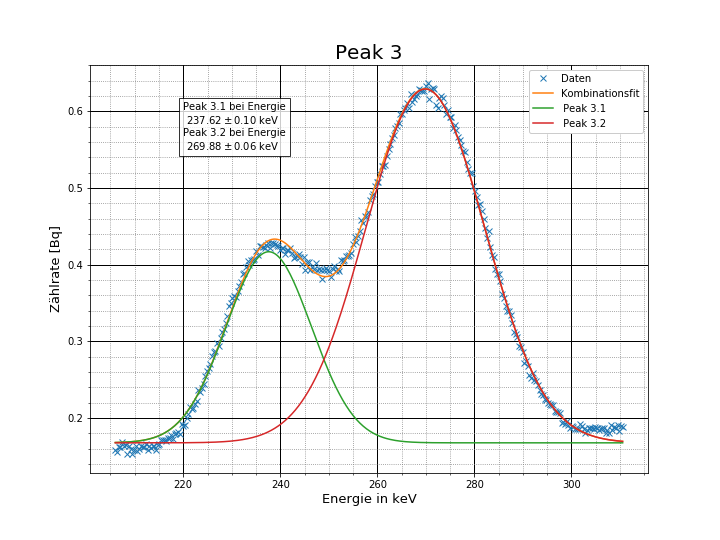
\includegraphics[scale=0.7]{Bilder/Anhang/P3}
	\caption[Thorium Peak 3]{\small Die verwendeten Daten von Peak 3, der gefittete Kombinationspeak, die einzelnen Peaks und ihre Mittelpunkte.}
	\label{p3}
\end{figure}

\subsubsection{Peak 4}
Das gefittete Maximum von Peak 4 liegt bei $345\pm0.23\,$ keV, was Abbildung \ref{p4} zu entnehmen ist. Es ist relativ offensichtlich, dass hier das echte Maximum der Daten neben dem des Fits liegt, weshalb für die Energie von Peak 4 der Wert $350\pm3\,$ keV angenommen wird. Vermutlich spielen hier außerdem Überlagerungen von Comptoneffekten der darüberlegenden Peaks eine Rolle, weshalb zusätzlich systematische Fehler anzunehmen sind \cite{staatsex_szinti}.\par
Hier existert kein Zerfall mit ähnlicher Energie zu Peak 4. Der nächste Übergang wäre der von Bismut zu Thallium bei einer Energie von 327.94 keV \cite{Bismut}. 
\begin{figure}[h]
	\centering
	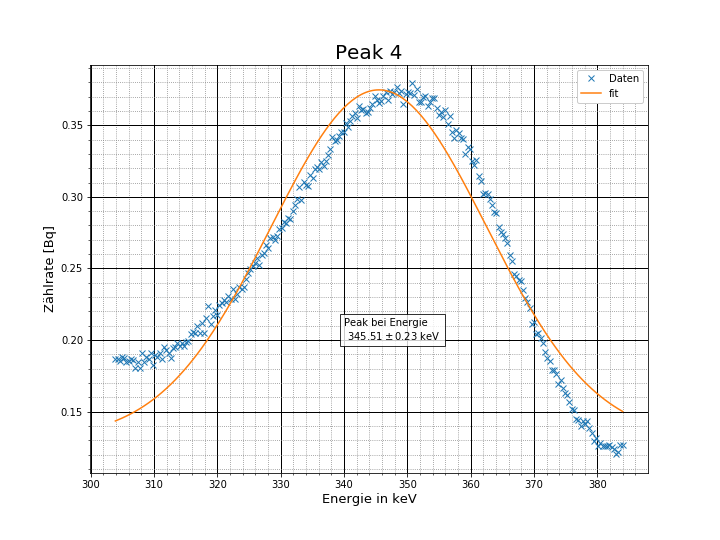
\includegraphics[scale=0.7]{Bilder/Anhang/P4}
	\caption[Thorium Peak 4]{\small Die verwendeten Daten von Peak 4, der gefittete Peak und sein Mittelpunkt.}
	\label{p4}
\end{figure}

\subsubsection{Peak 5}
Das gefittete Maximum von Peak 5 liegt bei $409.99\pm0.07\,$keV nach Abbildung \ref{p5}. Durch die hohe Streuung der Messwerte sollte ein höherer Fehler auf diesen Wert Angenommen werden, sodass für den Peak der Wert $410\pm2\,$keV gilt.\par
Hier wurde wahrscheinlich der Übergang von Blei zu Bismut mit einer Energie von 415.27 keV \cite{Blei} gemessen. 

\begin{figure}[h]
	\centering
	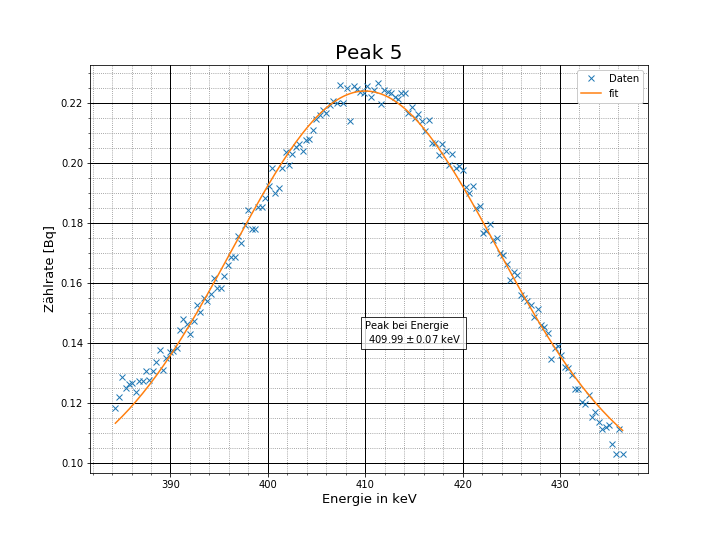
\includegraphics[scale=0.7]{Bilder/Anhang/P5}
	\caption[Thorium Peak 5]{\small Die verwendeten Daten von Peak 5, der gefittete Peak und sein Mittelpunkt.}
	\label{p5}
\end{figure}

\subsubsection{Peak 6}
Das gefittete Maximum von Peak 6 liegt bei $518.8\pm0.9\,$keV nach Abbildung \ref{p6}. Durch die hohe Streuung der Messwerte ist ein größerer Fehler auf diesen Wert angenommen worden, sodass für den Peak der Wert $519\pm5\,$keV gilt.\par
Wahrscheinlich wurde hier der 510.7 keV \cite{Thallium} Übergang von Thallium zu Blei gemessen.

\begin{figure}[h]
	\centering
	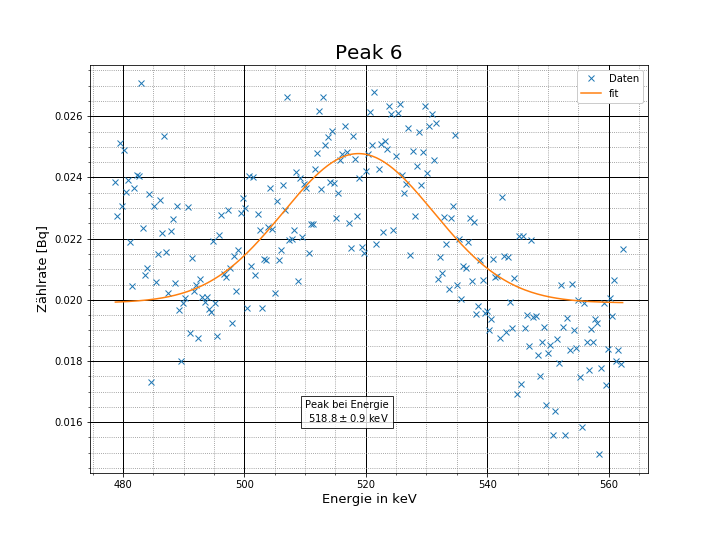
\includegraphics[scale=0.7]{Bilder/Anhang/P6}
	\caption[Thorium Peak 6]{\small Die verwendeten Daten von Peak 6, der gefittete Peak und sein Mittelpunkt.}
	\label{p6}
\end{figure}
\subsubsection{Peak 7}
Das gefittete Maximum von Peak 7 liegt bei $591.04\pm0.31\,$keV nach Abbildung \ref{p7}. Durch die hohe Streuung der Messwerte ist ein größerer Fehler auf diesen Wert angenommen worden, sodass für den Peak der Wert von $591\pm5\,$keV gilt.\par
Wahrscheinlich wurde hier der 587.8 keV \cite{Thallium} Übergang von Thallium zu Blei gemessen.

\begin{figure}[h]
	\centering
	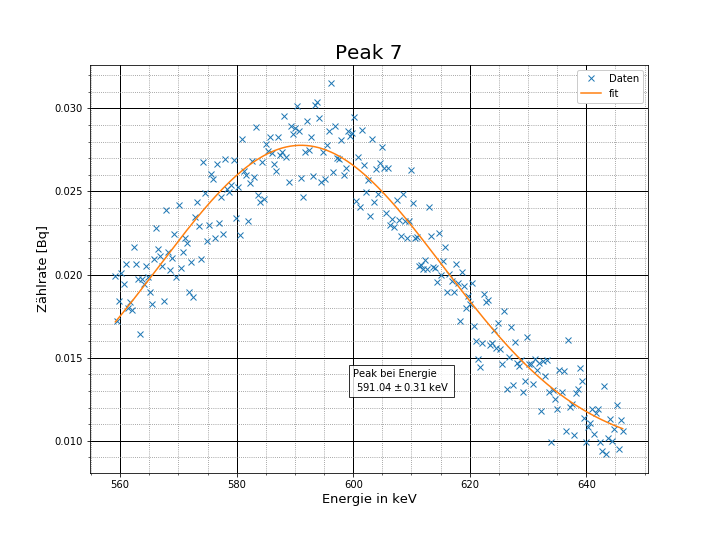
\includegraphics[scale=0.7]{Bilder/Anhang/P7}
	\caption[Thorium Peak 7]{\small Die verwendeten Daten von Peak 7, der gefittete Peak und sein Mittelpunkt.}
	\label{p7}
\end{figure}

\subsubsection{Peak 8}
Das gefittete Maximum von Peak 8 liegt bei $839.44\pm0.15\,$keV nach Abbildung \ref{p8}. Durch die hohe Streuung der Messwerte wurde ein größerer Fehler auf diesen Wert angenommen, sodass für den Peak ein Wert von $839\pm5\,$keV gilt.\par
Wahrscheinlich wurde hier der 835.9 keV \cite{Thallium} von Thallium zu Blei gemessen.

\begin{figure}[h]
	\centering
	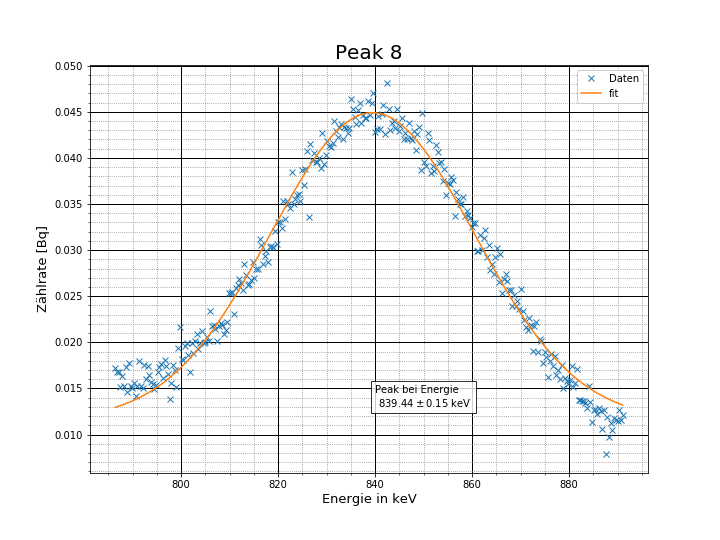
\includegraphics[scale=0.7]{Bilder/Anhang/P8}
	\caption[Thorium Peak 8]{\small Die verwendeten Daten von Peak 8, der gefittete Peak und sein Mittelpunkt.}
	\label{p8}
\end{figure}

\subsubsection{Peak 9}
Das gefittete Maximum von Peak 9 liegt bei $2614.1\pm0.5\,$keV nach Abbildung \ref{p9}. Durch die hohe Streuung der Messwerte wurde ein größerer Fehler auf diesen Wert angenommen, sodass für den Peak ein Wert von $2614\pm10\,$keV gilt.\par
Wahrscheinlich wurde hier der 2614.511 keV \cite{Thallium} Übergang von Thallium zu Blei gemessen.

\begin{figure}[h]
\centering
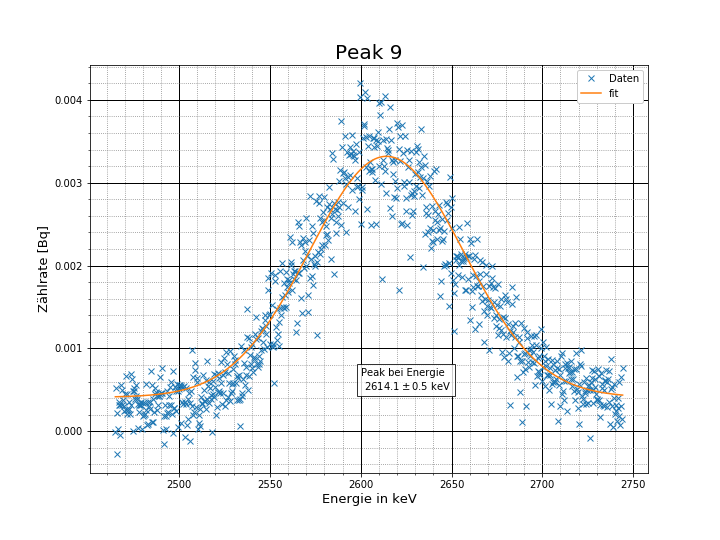
\includegraphics[scale=0.7]{Bilder/Anhang/P9}
\caption[Thorium Peak 9]{\small Die verwendeten Daten von Peak 9, der gefittete Peak und sein Mittelpunkt.}
\label{p9}
\end{figure}